\documentclass{article}
\usepackage[utf8]{inputenc}
\usepackage[spanish, es-tabla]{babel}
\usepackage{amsmath}
\usepackage{amsfonts}
\usepackage{siunitx}
\usepackage{amssymb}
\usepackage{graphics}
\usepackage{float}
\usepackage{lipsum}
\usepackage{multicol}
\usepackage{graphicx}
\usepackage{multirow}
\usepackage{wrapfig}
\usepackage{subcaption}
\usepackage[hidelinks]{hyperref}
\usepackage{enumitem}
\usepackage{graphicx}
\usepackage{mwe}
\usepackage{lipsum}
\usepackage{caption}
\usepackage{booktabs}

%-------Márgenes--------
\usepackage{geometry}
\newgeometry{
    left=2.54cm,
    right=2.54cm,
    top=2.4cm,
    bottom=2.4cm}
%-------Pie de Página--------
\usepackage{fancyhdr}
\pagestyle{fancy}
\fancyhf{}    % Quitar configuración por defecto
\renewcommand{\headrulewidth}{0pt}  %Quitar linea del encabezado
\cfoot[]{}   
\lfoot[]{\small \textit{Herramientas Computacionales, 2023} }
\rfoot[]{\textit{\thepage}}
\setcounter{page}{1}   %Numeración
%\usepackage{showframe}
%--------------------------------------------------------------

\author{J.P. Luengas^{1} , J.C. Aranda^{1}
}
\date{}
%===============================================================
% Inicio del documento
\begin{document}
 
     \begin{center}
    % TÍTULO DEL TRABAJO
        {\large\textbf{Implementación de la discretizacion de la ecuación de difusión por medio de diferencias finitas}}\\
        \vspace{5mm}
        % AUTORES 
        {\small \textbf{M.A. Garcia$^{1}$}, \textbf{M. García}$^{2}$}\\
        \vspace{3mm}
        % AUTORES 
        {\small \textit{Departamento de Física, Universidad Nacional de Colombia, Sede Bogotá, Bogotá, Colombia.}}\\
        \vspace{3mm}
        % FECHA 
        {\small 13/06/2023}
    \end{center}
    {\small \textit {Email: mangarciama@unal.edu.co$^{1}$, mgarciamej@unal.edu.co$^2$}} \\
    
    \vspace{5mm}

% RESUMEN
{\large \textbf{Resumen}}\\
En el presente texto se presenta un enfoque numérico para la resolución de la ecuación de difusión utilizando diferencias finitas. Se utiliza la primera ley de Fick para establecer la relación entre el flujo y el gradiente de concentración. Mediante la discretización de la ecuación, se divide el espacio y el tiempo en una malla de puntos y se aproximan las derivadas parciales. Esto conduce a un sistema de ecuaciones lineales que describe la evolución de la concentración a lo largo del tiempo. Los resultados demuestran que la aproximación numérica por diferencias finitas es una herramienta efectiva para simular procesos de difusión y transferencia de calor en diversas áreas científicas y tecnológicas.

 \textit{Palabras clave: enfoque numérico, ecuación de difusión, diferencias finitas, ley de Fick, discretización, simulación \hspace{2mm}}

\section{Deducción de la ecuación de difusión}
Sea una cantidad $u(\textbf{r},t)$ dependiente de su posición en el espacio ($\textbf{r}$) y el tiempo ($t$), donde $\textbf{r} = (x,y,x)$ representa vectorialmente su localización. Nuestro objetivo es describir el cambio de esta cantidad en el tiempo debido a la difusión. Para esto nos referimos a la primera ley de Fick, derivada empíricamente, la cual postula que el flujo de una sustancia se dirige de regiones con mayor concentración a regiones de menor concentración con una magnitud proporcional al gradiente de concentración. Esto lo podemos expresar:

\begin{equation}
    \textbf{J} = -D \cdot \nabla u(\textbf{r},t)
    \label{eq:fick1}
\end{equation}
Donde $\textbf{J}$ es el flujo de la cantidad y $D$ es el coeficiente de difusión, que se supone constante para que el proceso de difusión sea homogéneo en el espacio y tiempo. \\

Ahora, definamos una concentración local y flujo a través de una unidad de área $A$ en una posición $\textbf{r}$:

\begin{equation}
    du(\textbf{r}) = \frac{A \cdot [\textbf{J}(\textbf{r})-\textbf{J}(\textbf{r}+d\textbf{r})]}{A} \frac{dt}{d\textbf{r}}
\end{equation}
Y sabiendo que:
\begin{equation*}
    \textbf{J}(\textbf{r}+d\textbf{r}) = \textbf{J}(\textbf{r}) + d\textbf{J}
\end{equation*}
\begin{equation}
    \frac{\partial u(\textbf{r},t)}{\partial t} = -\frac{\partial \textbf{J}}{\partial x}
\end{equation}
Y recordando la primera ley (ec. \ref{eq:fick1}), reescribimos y encontramos la segunda ley de Fick, más conocida como la ecuación de difusión:
\begin{equation}
    \frac{\partial u(\textbf{r},t)}{\partial t} = -\frac{\partial }{\partial x} \left [ -D \cdot \nabla u(\textbf{r},t) \right ]
\end{equation}
\begin{equation}
    \frac{\partial u}{\partial t} = -D \cdot \nabla^2 u
    \label{eq:difusion}
\end{equation}


\section{Discretización de la ecuación de difusión por diferencias finitas}
Para resolver numéricamente la ecuación de difusión utilizando el método de diferencias finitas, es necesario discretizar tanto el dominio espacial como el temporal. A continuación, se describirá el procedimiento paso a paso para llevar a cabo esta discretización.

\subsection{Discretización del Dominio Espacial y Temporal}
El primer paso consiste en discretizar el dominio espacial en una malla de puntos equidistantes. Supongamos que tenemos un dominio unidimensional y consideremos un intervalo espacial de longitud \(L\) dividido en \(N+1\) puntos, donde \(N\) es el número total de puntos en la malla.

Denotemos por \(u_i\) la cantidad desconocida en el punto \(i\) de la malla, donde \(i = 0, 1, 2, \ldots, N\). Para cada punto \(i\), definimos su posición espacial como \(x_i = i \Delta x\), donde \(\Delta x = \frac{L}{N}\) es la distancia entre puntos adyacentes \cite{difusion_diferencias_finitas}.

\begin{figure}[H]
    \centering
   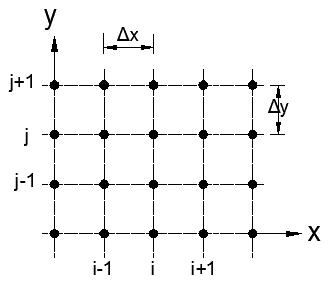
\includegraphics[width=0.3\textwidth]{Discretizacion_dominio_espacial.png}
    \caption{Diagrama de la discretizacion del dominio espacial para el metodo de diferencias finitas \cite{diagrama_discretizacion}.}
    \label{fig:discretizacion_espacial}
\end{figure}

Una vez que hemos discretizado el dominio espacial, procedemos a discretizar el dominio temporal. Dividimos el intervalo temporal de interés en \(M\) intervalos igualmente espaciados, donde \(M\) es el número total de pasos de tiempo.

Denotemos por \(u_i^m\) el valor aproximado de la cantidad \(u\) en el punto \(i\) de la malla en el paso de tiempo \(m\), donde \(m = 0, 1, 2, \ldots, M\). Definimos el tiempo en el paso \(m\) como \(t_m = m \Delta t\), donde \(\Delta t\) es el tamaño del paso de tiempo \cite{difusion_diferencias_finitas}.

\subsection{Aproximación de las Derivadas Parciales}

Para discretizar las derivadas parciales en la ecuación de difusión, utilizamos aproximaciones de diferencias finitas. Existen diferentes esquemas de aproximación, siendo los esquemas explícito e implícito los más comunes.

\subsubsection{Esquema Explícito}
En el esquema explícito, aproximamos la derivada temporal por una diferencia hacia adelante y la derivada espacial por una diferencia central. La discretización de la ecuación de difusión en el punto \((i,m)\) utilizando este esquema se puede expresar de la siguiente manera \cite{difusion_diferencias_finitas}:

\[
\frac{T_i^{m+1} - T_i^m}{\Delta t} = D \left( \frac{T_{i+1}^m - 2T_i^m + T_{i-1}^m}{(\Delta x)^2} \right)
\]

donde \(D\) es el coeficiente de difusión.


\subsubsection{Esquema Implícito}
En el esquema implícito, aproximamos tanto la derivada temporal como la derivada espacial por diferencias centrales. La discretización de la ecuación de difusión en el punto \((i,m)\) utilizando este esquema se puede expresar de la siguiente manera \cite{difusion_diferencias_finitas}:

\[
\frac{T_i^{m+1} - T_i^m}{\Delta t} = D \left( \frac{T_{i+1}^{m+1} - 2T_i^{m+1} + T_{i-1}^{m+1}}{(\Delta x)^2} \right)
\]

\subsection{Formulación del Sistema de Ecuaciones}

Una vez que hemos aproximado las derivadas parciales, podemos reorganizar las ecuaciones discretizadas y obtener un sistema de ecuaciones lineales. Esto se logra agrupando los términos correspondientes a cada punto \(i\) y cada paso de tiempo \(m\).

En el caso del esquema explícito, el sistema de ecuaciones resultante es:

\begin{gather}
T_i^{m+1} = T_i^m + \frac{D \Delta t}{(\Delta x)^2} (T_{i+1}^m - 2T_i^m + T_{i-1}^m)
\label{ec:discretizacion_explicita}
\end{gather}

En el caso del esquema implícito, el sistema de ecuaciones resultante es:

\[
T_i^{m+1} - \frac{D \Delta t}{(\Delta x)^2} (T_{i+1}^{m+1} - 2T_i^{m+1} + T_{i-1}^{m+1}) = T_i^m
\]

\section{Aproximación numérica de la ecuación de difusión por diferencias finitas}
Utilizando las librerías Numpy y Matplotlib se implementó la solución numérica a la ecuación de difusión (ec. \ref{ec:discretizacion_explicita}) con un coeficiente de difusión constante y arbitrario en distribuciones de concentración centradas en el espacio y conservando dos simetrías: polar y cuadrada; el codigo utilizado para realizar las imagenes se puede encontrar en \href{https://github.com/alhazacod/heat_eq_t_dependant_boundary}{GitHub} o en el siguiente link: \url{https://github.com/alhazacod/heat_eq_t_dependant_boundary}. Una posible aplicación de esta solución es el derretimiento de un bloque de hielo en forma cilíndrica o cúbica.

\subsection{Distribución con simetría polar}
A continuación se muestra la evolución temporal de la solución numérica obtenida en el caso con simetría polar:

\begin{figure} [H]
  \centering
  \begin{subfigure}{0.25\linewidth}
    \centering
    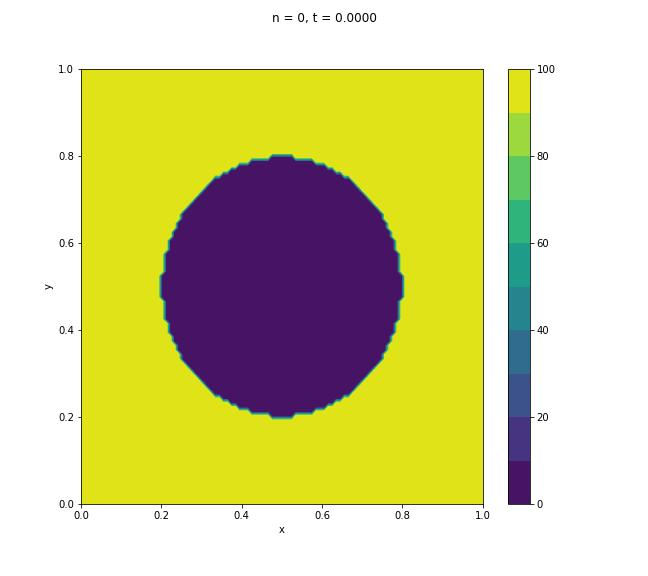
\includegraphics[width=\linewidth]{Polar/2D/0.jpg}
    \caption{Frame 0}
  \end{subfigure}
  \begin{subfigure}{0.25\linewidth}
    \centering
    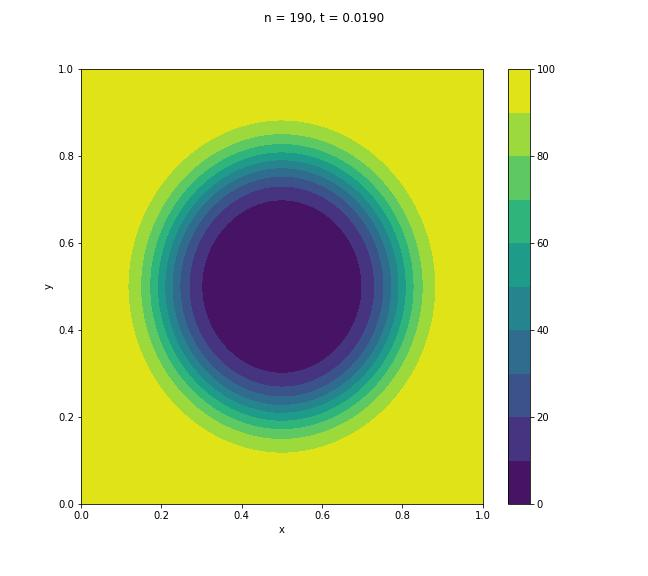
\includegraphics[width=\linewidth]{Polar/2D/190.jpg}
    \caption{Frame 190}
  \end{subfigure}
  \begin{subfigure}{0.25\linewidth}
    \centering
    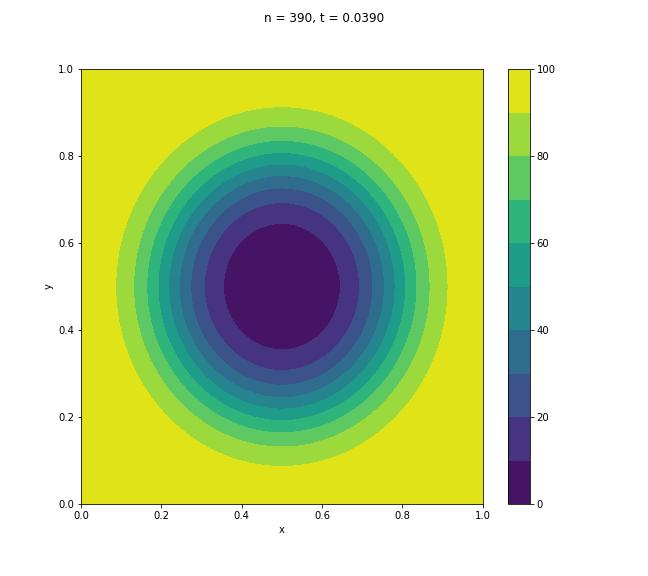
\includegraphics[width=\linewidth]{Polar/2D/390.jpg}
    \caption{Frame 390}
  \end{subfigure}
    \begin{subfigure}{0.25\linewidth}
    \centering
    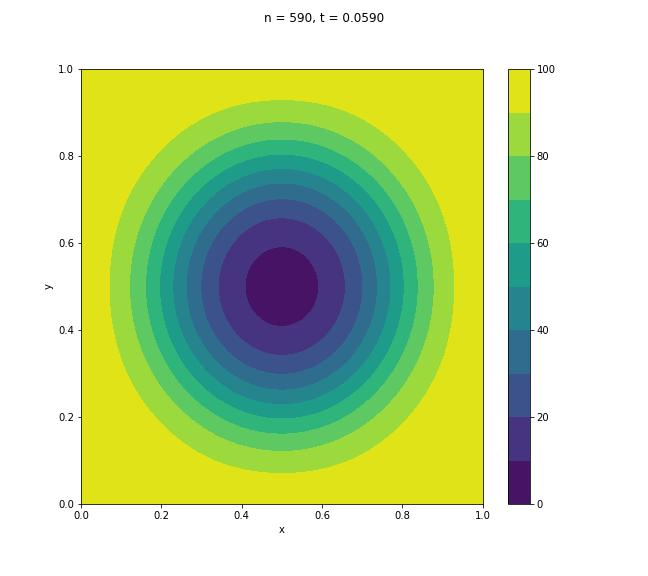
\includegraphics[width=\linewidth]{Polar/2D/590.jpg}
    \caption{Frame 590}
  \end{subfigure}
      \begin{subfigure}{0.25\linewidth}
    \centering
    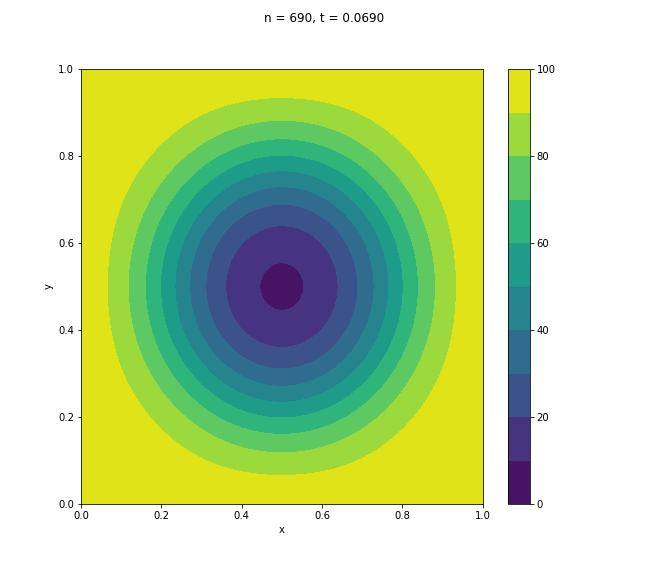
\includegraphics[width=\linewidth]{Polar/2D/690.jpg}
    \caption{Frame 690}
  \end{subfigure}
      \begin{subfigure}{0.3\linewidth}
    \centering
    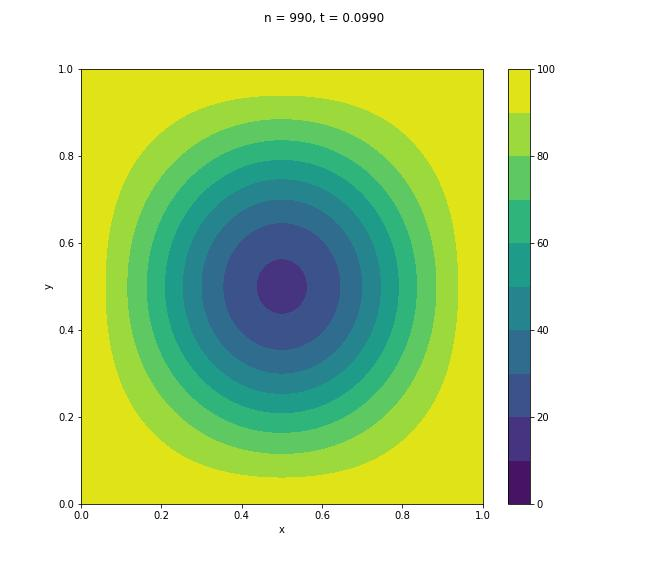
\includegraphics[width=\linewidth]{Polar/2D/990.jpg}
    \caption{Frame 990}
  \end{subfigure}
  \caption{Distribución de concentración función del tiempo}
  \label{fig:polar2d}
\end{figure}

Continuando con la aplicación mencionada anteriormente, también posible visualizar en tres dimensiones el derretimiento el hielo con simetría cilíndrica:

\begin{figure} [H]
  \centering
  \begin{subfigure}{0.3\linewidth}
    \centering
    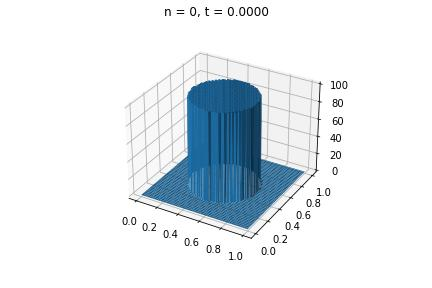
\includegraphics[width=\linewidth]{Polar/3D/0.jpg}
    \caption{Frame 0}
  \end{subfigure}
  \begin{subfigure}{0.3\linewidth}
    \centering
    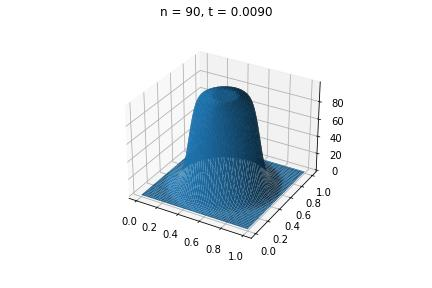
\includegraphics[width=\linewidth]{Polar/3D/90.jpg}
    \caption{Frame 90}
  \end{subfigure}
  \begin{subfigure}{0.3\linewidth}
    \centering
    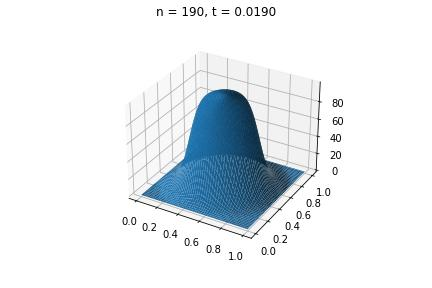
\includegraphics[width=\linewidth]{Polar/3D/190.jpg}
    \caption{Frame 190}
  \end{subfigure}
  \begin{subfigure}{0.3\linewidth}
    \centering
    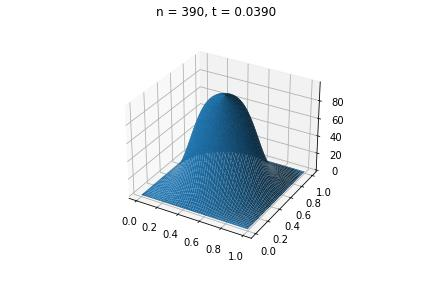
\includegraphics[width=\linewidth]{Polar/3D/390.jpg}
    \caption{Frame 390}
  \end{subfigure}
    \begin{subfigure}{0.3\linewidth}
    \centering
    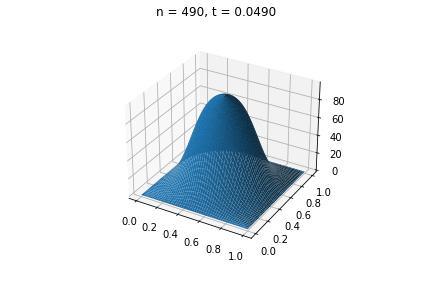
\includegraphics[width=\linewidth]{Polar/3D/490.jpg}
    \caption{Frame 490}
  \end{subfigure}
      \begin{subfigure}{0.3\linewidth}
    \centering
    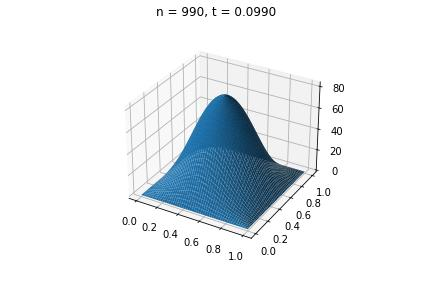
\includegraphics[width=\linewidth]{Polar/3D/990.jpg}
    \caption{Frame 990}
  \end{subfigure}
  \caption{Distribución de concentración función del tiempo}
  \label{fig:cilindrica3d}
\end{figure}

\subsection{Distribución con simetría cuadrada}
Por otra parte, a continuación tenemos la evolución temporal con simetría cuadrada:

\begin{figure} [H]
  \centering
  \begin{subfigure}{0.25\linewidth}
    \centering
    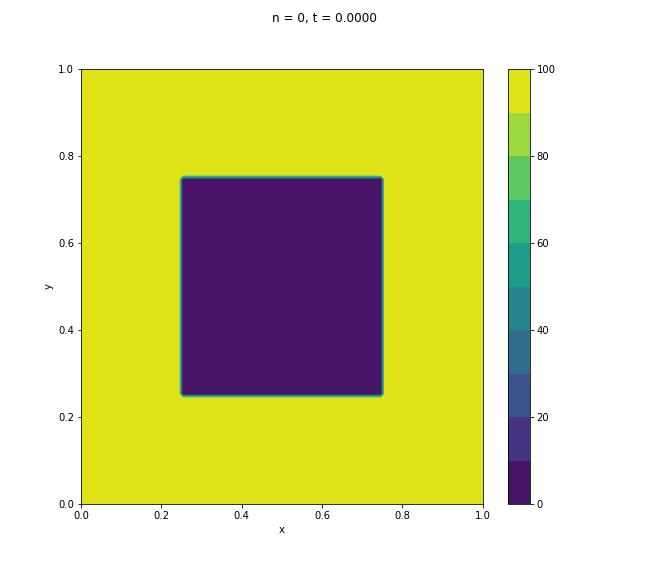
\includegraphics[width=\linewidth]{Cuadrada/2D/0.jpg}
    \caption{Frame 0}
  \end{subfigure}
  \begin{subfigure}{0.25\linewidth}
    \centering
    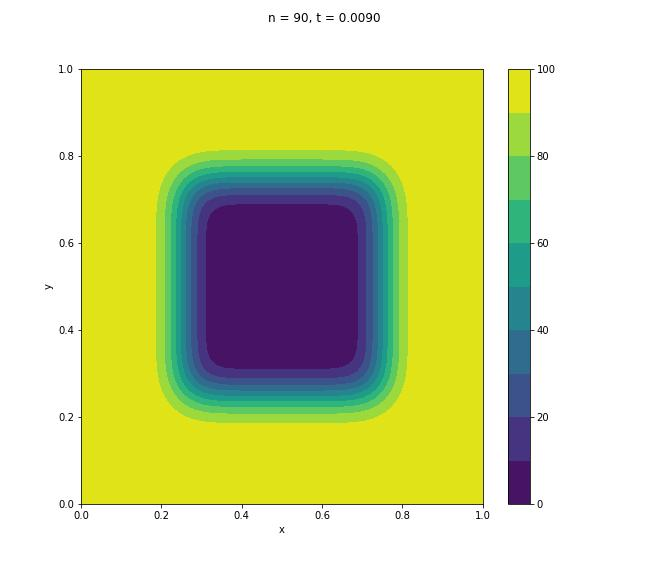
\includegraphics[width=\linewidth]{Cuadrada/2D/90.jpg}
    \caption{Frame 90}
  \end{subfigure}
  \begin{subfigure}{0.25\linewidth}
    \centering
    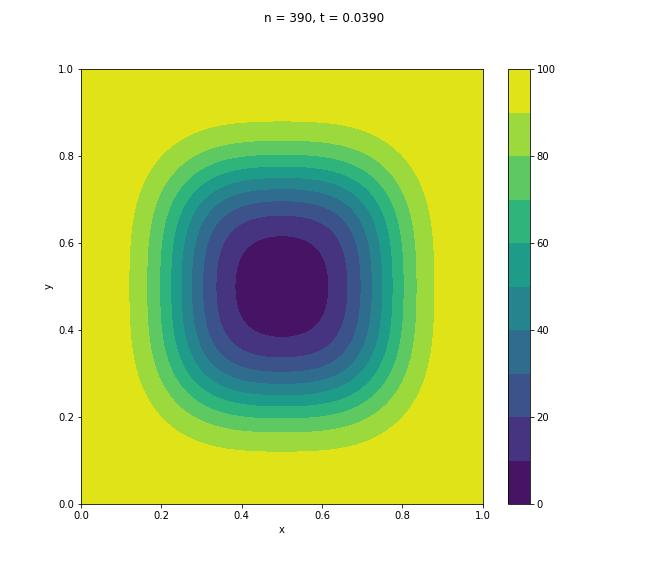
\includegraphics[width=\linewidth]{Cuadrada/2D/390.jpg}
    \caption{Frame 390}
  \end{subfigure}
    \begin{subfigure}{0.25\linewidth}
    \centering
    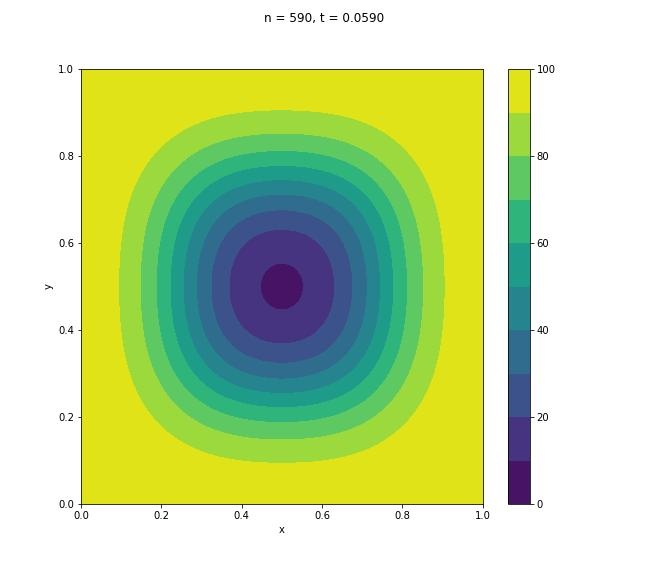
\includegraphics[width=\linewidth]{Cuadrada/2D/590.jpg}
    \caption{Frame 590}
  \end{subfigure}
      \begin{subfigure}{0.25\linewidth}
    \centering
    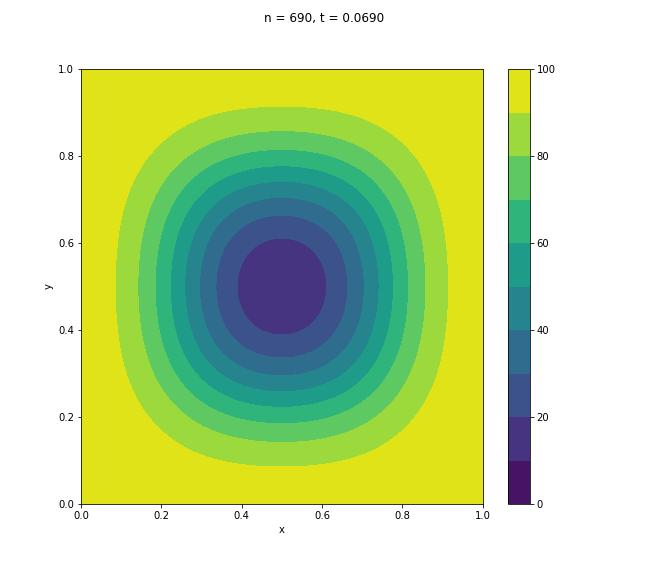
\includegraphics[width=\linewidth]{Cuadrada/2D/690.jpg}
    \caption{Frame 690}
  \end{subfigure}
      \begin{subfigure}{0.25\linewidth}
    \centering
    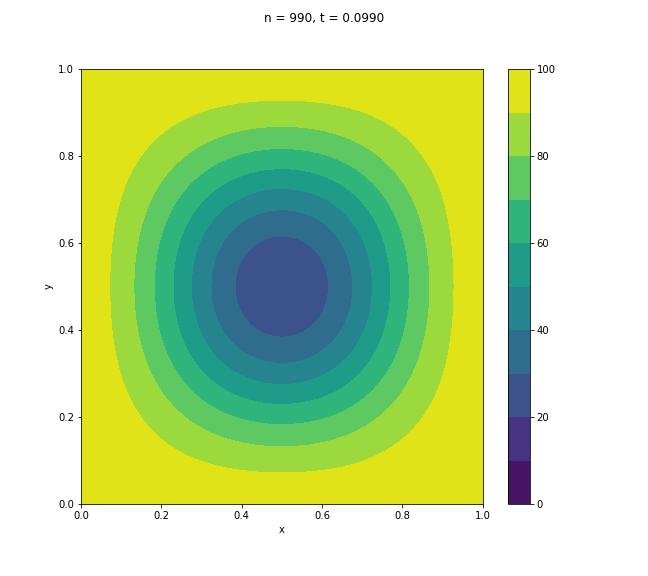
\includegraphics[width=\linewidth]{Cuadrada/2D/990.jpg}
    \caption{Frame 990}
  \end{subfigure}
  \caption{Distribución de concentración función del tiempo}
  \label{fig:cuadrada2d}
\end{figure}

Y el caso del derretimiento de un cubo de hielo:

\begin{figure} [H]
  \centering
  \begin{subfigure}{0.3\linewidth}
    \centering
    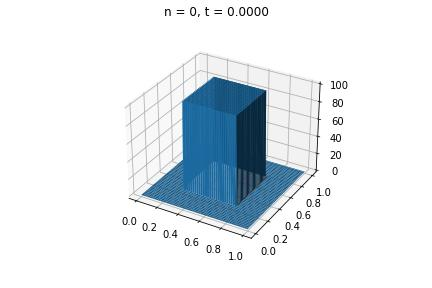
\includegraphics[width=\linewidth]{Cuadrada/3D/0.jpg}
    \caption{Frame 0}
  \end{subfigure}
  \begin{subfigure}{0.3\linewidth}
    \centering
    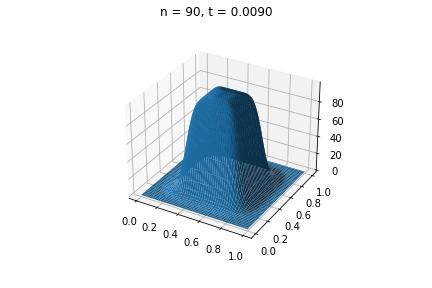
\includegraphics[width=\linewidth]{Cuadrada/3D/90.jpg}
    \caption{Frame 90}
  \end{subfigure}
  \begin{subfigure}{0.3\linewidth}
    \centering
    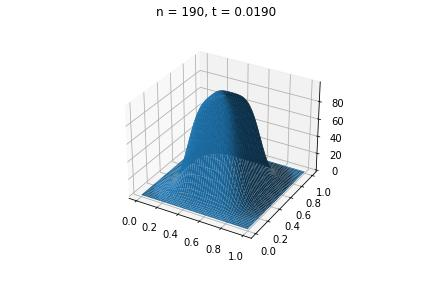
\includegraphics[width=\linewidth]{Cuadrada/3D/190.jpg}
    \caption{Frame 190}
  \end{subfigure}
  \begin{subfigure}{0.3\linewidth}
    \centering
    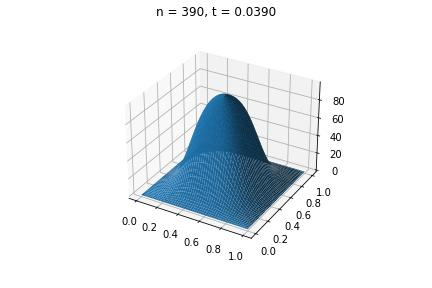
\includegraphics[width=\linewidth]{Cuadrada/3D/390.jpg}
    \caption{Frame 390}
  \end{subfigure}
    \begin{subfigure}{0.3\linewidth}
    \centering
    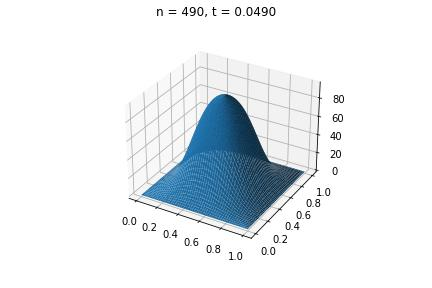
\includegraphics[width=\linewidth]{Cuadrada/3D/490.jpg}
    \caption{Frame 490}
  \end{subfigure}
      \begin{subfigure}{0.3\linewidth}
    \centering
    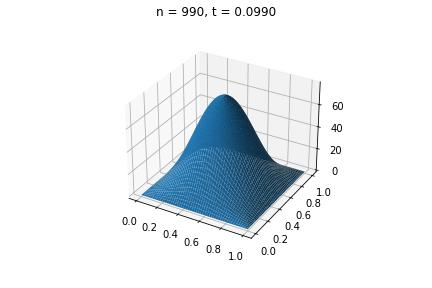
\includegraphics[width=\linewidth]{Cuadrada/3D/990.jpg}
    \caption{Frame 990}
  \end{subfigure}
  \caption{Distribución de concentración función del tiempo}
  \label{fig:cubica3d}
\end{figure}

\section{Conclusiones}
En conclusión, hemos realizado la deducción de la ecuación de difusión utilizando la primera ley de Fick, estableciendo la relación entre el flujo de una cantidad y el gradiente de concentración. Posteriormente, hemos discretizado la ecuación de difusión por diferencias finitas, dividiendo el dominio espacial y temporal en una malla de puntos equidistantes y aproximando las derivadas parciales mediante esquemas explícitos e implícitos. Esto nos ha permitido formular un sistema de ecuaciones lineales que representa la evolución de la concentración en el tiempo.\\

La aproximación numérica de la ecuación de difusión por diferencias finitas ha demostrado ser una herramienta efectiva para simular el proceso de difusión en sistemas físicos. Mediante la discretización del dominio espacial y temporal, y la aproximación de las derivadas parciales, hemos obtenido soluciones numéricas que muestran la evolución de la concentración en el tiempo para diferentes distribuciones iniciales con simetrías polar y cuadrada. Estas soluciones nos brindan información visual sobre el comportamiento de la difusión, permitiéndonos analizar el derretimiento de un bloque de hielo y observar cómo la concentración se distribuye de manera gradual a lo largo del tiempo. Esta aproximación numérica por diferencias finitas es ampliamente utilizada en diversos campos científicos y tecnológicos para estudiar procesos de difusión y transferencia de calor.



\begin{thebibliography}{X}

    \bibitem{difusion_diferencias_finitas} William H. Press, Saul A. Teukolsy, William T. Vetterling, Brian P. Flannery, (2007). \textit{Numerical Recipes: The Art of Scientific Computing} Cap. 20.

    \bibitem{diagrama_discretizacion}Ossa, Alexandra and Zapata, Verónica and Botero-Jaramillo, Eduardo, (2015). \textit{METODOLOGÍA PARA RESOLVER POR DIFERENCIAS FINITAS NUEVOS MODELOS CONSTITUTIVOS EN EL PROGRAMA FLAC3D}

    \bibitem{robertson} David G. Robertson (2010). \textit{Relaxation Methods for Partial Differential Equations: Applications to Electrostatics}. Department of Physics and Astronomy, Otterbein University.
    
 \end{thebibliography}

\end{document}